\chapter{Entwicklung}
In diesem Kapitel werden die einzelnen Komponenten, die für eine komplette Ingestion notwendig sind entwickelt.
Nach \citeauthor{DL-Ing-Mgmt} ist der Ingestion-Prozess eines Data-Lake-Systems, als erster Schritt im Lebenszyklus der Daten, maßgebend dafür, wie gut die Daten später verwendet und verarbeitet werden können.
Um diese Aufgabe so gut wie möglich zu erfüllen, wurden im vorherigen Kapitel bereits die Anforderung festgelegt.
Daraus ergeben sich die drei Inhaltlichen Bereiche, nach denen die weiter Entwicklung aufgeteilt ist.

Der erste ist die Ingestion.
Diese beschreibt das erfassen von Informationen über eine Datenquelle und das Laden der Daten aus der Datenquelle.
Dabei werden die Daten noch nicht intern im Data Lake wieder abgelegt sondern existieren nur flüchtig im Arbeitsspeicher.

Die Deltaerkennung ist dafür zuständig die Unterschiede zwischen den geladenen Daten im Arbeitsspeicher und den aktuellen Daten aus dem internen Data Lake Speicher zu finden.
Aus diesen Unterschieden sollen die Änderungsdaten erstellt werden, die dann bei der weiteren Verarbeitung verwendet werden können.

Der dritte Bereich ist das Speichern von Daten in einem vordefinierten als auch in einem frei bestimmbaren Speichersystem zählt.
Der Unterschied dabei ist, dass im vordefinierten Speicher die Datenversionierung durch das Data-Lake-System unterstützt wird, während dies bei frei wählbaren nicht der Fall ist.

\section{Architektur}
\label{sec:arch}

Zu Anfang ist es sinnvoll, die Architektur des Systems festzulegen.
Diese bestimmt, welche Komponenten und Microservices entwickelt und verbunden werden müssen.
Der erste Schritt dabei ist es, die Aufagben aufzuteilen, die das System erfüllen soll.
Diese Aufgaben werden dann auf Microservices verteilt und in einer Architektur verbunden.
Die weitere Entwicklung des Systems stützt sich dann auf die fertige Architektur.

\subsection{Aufgabenverteilung}
Durch die Verwendung von \textit{Apache Spark} ist es nicht sinvoll, dass Laden der Daten, die Deltaerkennung und das Speichern zu trennen.
In \textit{Apache Spark} werden alle drei Arbeitsschritte auf einem \verb|Dataframe| ausgeführt.
Das heißt, dass dieses zwischen den Microservices ausgetauscht werden müsste, was zu einem erheblichen Aufwand führen würde.
Aus diesem Grund können die drei Bereiche aus der Einleitung nicht auch als Aufgabenverteilung verwendet werden.

Besser trennbare Aufgaben findet man bei der Betrachtung der technischen Seite.
Hierbei gibt es die Api, die Ingestion in \textit{Apache Spark} und das kontunierliche Ausführen.

Bei der \textbf{Api} handelt es sich um den Server für die Interaktion mit dem Data Lake System.
Durch die Anforderungen ist bereits festgelegt, dass dieser ein Web-Server mit einer REST-Schnittstelle ist.
Es geht zwar in dieser Arbeit nur um die Ingestion, aber diese Api kann für alle Funktionen des Datalakes verwendet werden.

Die \textbf{Ingestion} ist dafür zuständig, die Datenquellen zu verarbeiten und den kompletten Prozess von Laden bis Speichern der Daten in \textit{Apache Spark} auszuführen.
Die Ausführung soll für eine Datenquelle nur einmal gleichzeitig aber parallel für unterschiedliche laufen.

Bei einer zeitgesteuerten oder Datenstrom-Ingestion, muss die \textbf{kontinuierliche Ausführung} sichergestellt werden.
Für alle Datenquellen muss regelmäßig geprüft werden, ob für diese gerade eine Ingestion ausgeführt wird und ausgeführt werden sollten.
Falls keine ausgeführt wird aber sollte, wird die Ingestion für diese Datenquelle.

\subsection{Komponenten und Microservices}
Jede dieser Aufgaben kannn einem Microservice zugeordnet werden.
In \fref{fig:ingestion_arch} ist eine Architektur zu sehen, die Microservices für jede dieser aufgaben beinhaltet.
Der Api-Server übernimmt die REST-Schnittstelle, der Ingestion-Server kümmert sich um die Ausführung der Ingestion und der Continuation-Server stellt die kontinuierliche Ausführung sicher.

Neben diesen drei wird noch ein Nachrichtensystem benötigt, das dafür zuständig ist, die Kommunikation zwischen den  einzelnen Microservices zu koordinierten.
Dabei werden Nachrichten nicht direkt an einen anderen Mircoservices gesendet, sonder unter einem bestimmten Schlüssel an das Nachrichtensystem.
Das kümmert sich dann darum, dass alle Microservices, die Nachrichten mit diesem Schlüssel empfangen wollen, diese auch bekommen.
Ein Vorteil dabei ist, dass es sowhl einfach wird, einzelne Mircoservices horizontal zu skalieren, als auch neue in das System zu integrieren.

Zum Ablegen der internen Informationen wird eine Datenbank benötigt.
Alle Microservices haben zugriff auf diese Datenbank und können Daten in ihr beareiten.
Es handelt sich dabei aber nicht um den internen Speicher des Data Lakes sondern nur um Daten, die für den Betrieb des Systems benötigt werden.
Darunter fallen zum Beispiel Authentifizierungsdaten oder Verbindungsinformationen von Datenquellen.

\begin{figure}
  \centering
  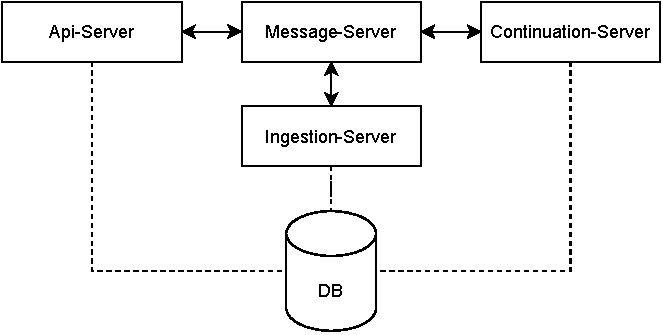
\includegraphics{Grafiken/ingestion-arch.pdf}
  \caption{Architektur der Ingestion Komponenten}
  \label{fig:ingestion_arch}
\end{figure}


\subsection{Datenquellen}
Ein weiterer Kernpunkt der Ingestion-Schnittstelle ist die Modellierung der Datenquellen.
Um ein Datenmodel zu entwicklen, werden zuerst die möglichen Datenquellen analysiert.
Aus dieser Analyser werden dann Informationen erstellt, die das System über die Datenquelle wissen muss.
Das daraus enstandene Model wird dann um alle Informationen erweitert, die für den Betrieb oder die Benutzung des Systems hilfreich sind.

Da das System alle möglichen Datenquellen unterstützen soll, werden hier mögliche Typen dargestellt, mit denen sich alle Datenquellen abdecken lassen.
Dazu werden Merkmale betrachtet die Art und der Typ Ingestion bestimmen.
Mit der Art wird hier bezeichnet, ob die verwendeten Daten strukturiert, semi- oder unstrukturiert sind.
Da in der Vorarbeit, dem Masterprojekt, \textit{Apache Spark} verwendet wurde, ist dieser Punkt bereits abgedeckt und fällt bei der Entwicklung nicht weiter ins Gewicht.

Als zweites gibt es die Typen, die hier beschreiben, wie Daten in das System gelangen.
Dazu gibt es zwei Merkmale, in denen sich die Ingestions unterscheiden können.
Das erste ist, ob die Unterscheidung zwischen Push- und Pull-Prinzip.
Bei dem Push-Prinzip werden die zu speichernden Daten mit der Anfrage an das System gesendet und bei dem Pull-Prinzip muss dass System die Daten aus einer Quelle laden.
Die zweite Unterscheidung findet statt in einmalige in kontinuierliche Ingestion.
Diese Unterscheidungen können, müssen aber nicht, von der Datenquelle abhängig sein.
Als Beispiel gibt es Datenströme, die laufend Daten senden und somit eine Ingestion benötigen, die auch laufend Daten annimmt.
Im Gegensatz dazu gibt es Datenbanken, bei denen das System die Daten aus der Quelle laden muss und somit die Ingestion sowohl einmalig als auch kontinuierlich sein kann.

Aus diesen Unterscheidungen ergeben sich die vier mögliche Verarbeitungswege, die in \ref{fig:ingestion_types} zu sehen sind.
Sowohl für Push- und Pull-Prinzip kann eine einfache Ingestion ausgeführt werden, die sich für kontinuierliche Pull-Ingestions wiederholt.
Bei einer kontinuierlichen Ingestion, bei der Daten an das System gesendet werden, handelt es sich um Datenströme, die eine extra Verarbeitung erfordern.

\begin{figure}
  \centering
  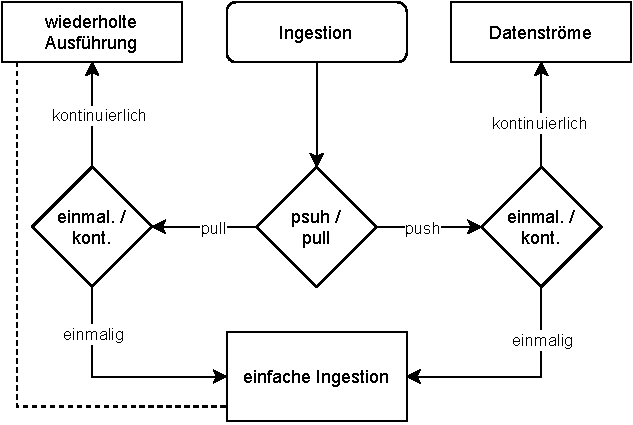
\includegraphics{Grafiken/ingestion-types.pdf}
  \caption{Ingestion-Typen}
  \label{fig:ingestion_types}
\end{figure}



\section{Vorüberlegungen}

Vor der Entwicklung der eigentlichen drei Komponenten, werden erst einige nötige Vorüberlegungen gemacht.
Diese beschäftigen sich genauer damit, wie genau Datenquellen zu definieren sind, wie das einbringen von eigenem Code funktionieren kann.




Bei der Ingestion soll der Teil entwickelt werden, der dafür verantwortlich ist, Daten aus verschiedensten Quellen in das Data-Lake-System zu laden und zu speichern.
Die Delta-Erkennung ist ein Mechanismus, der dafür sorgen soll, dass bei einer kontinuierlichen Ingestion nur geänderte Daten neu in das System integriert werden.
Zum Schluss hat die Datenversionierung das Ziel, geänderte Daten im Data Lake so zu verwalten, dass Analysen über den Verlauf der Daten und Abfragen älterer Version möglich werden.


\section{Ingestion}
Bei der Entwicklung der Ingestion wird das Laden der Daten und die Architektur der Anwendung betrachtet.
Es wird eine Datenmodell, in dem die Informationen zu den Datenquellen gespeichert werden, der Ablauf der verschiedenen Ingestion-Prozesse und die Kommunikation zwischen den einzelnen Mircoservices entwickelt.

\subsection{Server Architektur}

Für die Umsetzung der Mircoservice-Architektur wird die Ingestion in Komponenten aufgeteilt, die \fref{fig:ingestion_arch} zu sehen sind.
Es gibt drei Services, die für die Ingestion spezifischen Aufgaben zuständig sind, eine Datenbank, in der die Informationen über Datenquellen gespeichert werden und einen Service, der für die Kommunikation verantwortlich ist.
Der \textbf{Api-Server} bietet einen REST-Schnittstelle, über die man mit der Ingestion interagieren kann.
Hier werden die Endpunkte aus \fref{tab:enpoints} benötigt, die die Schnittstellen zur Verwaltung von Datenquellen und das Ausführen von Ingestions bereitstellen.
Außerdem ist er dafür zuständig, die empfangenen Informationen über Datenquellen in der Datenbank zu verwalten.
der \textbf{Continuation-Server} überprüft regelmäßig alle kontinuierlichen Datenquellen, ob diese eine Zeitsteuerung haben und aktuell ausgeführt werden sollten.
Der \textbf{Ingestion-Server} ist die Anwendung, die die eigentliche Ingestion ausführt.
Dafür wartet dieser auf eine Aufforderung durch entweder den Api- oder den Continuation-Server.

\begin{table}[!ht]
  \centering
  \begin{tabular}{| l | l | p{3in} |}
    \hline
    Pfad                                      & HTTP-Methode & Beschreibung                                                          \\
    \hline \hline
    /datasources                              & GET          & Liefert alle im System gespeicherten Datenquellen                     \\
    \hline
    /datasources/\textless id\textgreater     & GET          & Liefert die Datenquelle mit der im Pfad übergebenen Id                \\
    \hline
    /datasources                              & POST         & Erstellt eine neue Datenquelle                                        \\
    \hline
    /datasources/\textless id\textgreater     & PUT          & Bearbeitet die Daten Datenquelle mit der im Pfad übergebenen Id       \\
    \hline
    /datasources/\textless id\textgreater/run & GET          & Startet eine Ingestion der Datenquelle mit der im Pfad übergebenen Id \\
    \hline
  \end{tabular}
  \caption{Endpunkte des Api-Servers}
  \label{tab:enpoints}
\end{table}

\subsection{Plugins}
Da bei manchen Ingestions nicht immer ein festgelegtes Vorgehen ausreicht, um die Daten aus bestimmten Datenqellen zu laden, muss ein System entwickelt werden, wie möglichst ohne großen Aufwand die Inegstion erweitert werden kann.
Beispiele für solche Fälle sind die Verarbeitung von Datenströmen oder die Ingestion von Daten aus APIs, die nicht generallisiert werden können.
Als Lösung für das Problem, können Plugins der Datenquelle hinzugefügt werden.
Diese Plugins sollen Logik enthalten, die an verschiedenen Stellen der Ingestion ausgeführt werden sollen.
Aktuell sind diese Stellen das Laden der Daten, nach dem Laden der Daten und die Stream-Verarbeitung.
Dabei ist zu beachten, dass Plugins, die das Laden der Daten abhandeln, das Standardverhalten des Ingestion-Servers überschreiben und das Stream-Verarbeitung nur mit Plugins möglich ist.
Damit es nicht zu Konflikten bei Abhängigkeiten der Plugins gibt, muss der Ingestion-Server eine Mechanik implementieren, bei der die Abhängigkeiten der Plugins für jede Datenquelle dynamisch gealden werden.


\section{Deltaerkennung}